% You should title the file with a .tex extension (hw1.tex, for example)
\documentclass[11pt]{article}

\usepackage{bmpsize}
\usepackage[pdftex]{graphicx}
\usepackage{amsmath}
\usepackage{amssymb}
\usepackage{amsthm}
\usepackage{fancyhdr}
\usepackage[margin=2.5cm]{geometry}
\newcommand{\Ohm}{\Omega}
\newcommand{\inv}{^{-1}}
\renewcommand{\part}[1] {\vspace{.10in} {\bf (#1)}}


\pagestyle{fancyplain}


\begin{document}
\title{Digital Lab}
\author{David Galbraith}
\maketitle
%COMMENT: In Latex, using the maketitle function will perform all the formatting
%you had set up in the code below in a standard fashion

%\huge{Building an Amplifed FM Radio and Measuring Noise}\\
%\begin{center}
%\large{-----By David Galbraith-----}
%\end{center}


\normalsize
\begin{abstract}  %Abstract: \\

For this lab, we covered a wide range of topics relevant to digital
radio. I don't know what the hell they were yet though. %TODO: Figure
                                %out what the hell they were

\end{abstract}
%COMMENT: It is customary to use the abstract environment for the
%abstract, and to not include a pagebreak after the abstract prior to
%the introduction in a scientific paper


\lhead{\fancyplain{}{\textbf{Lab 2}}}      % Note the different brackets!
\rhead{\fancyplain{}{David Galbraith}}
\medskip                        % Skip a "medium" amount of space
                                % (latex determines medium is)
                                % Also try: \bigskip, \littleskip

\thispagestyle{plain}

\section{Introduction}
%COMMENT: Sections and subsections have their own format that will make
%the divisions in what you wrote more clear, and will number themselves,
%allowing you to focus more on content rather than order
The foremost, most fundamental piece of physics relevant to digital
signal sampling is the Nyquist criterion. A signal is a
continuously-varying quantity, but a computer can only read its value a
finite number of times. The Nyquist criterion states that in order to
get sample data that approximates the actual shape of the signal, one
must sample at at least twice the frequency of the signal.  

Digital shit is pretty sweet!! %TODO: Figure out what is sweet about it.


\section{Experiments, Observations, Analysis and Interpretation} 


%COMMENT: Using \label{value} and \ref{value} will allow you to refer to
%a specific figure without worrying about the order in which you have
%them in your document. While this obviously matters somewhat in terms
%of the logical flow of you paper, it's really helpful if you're moving
%things around as you write your paper. I did this for the first figure,
%but you can change the rest fairly easily. Additionally, \centering
%will put the figure in the middle of the page when you scale it down to
%a more reasonable size.

\subsection{The Nyquist Frequency}

The first thing we did in this lab was try to understand and visualize
the Nyquist criterion. To do this, we sampled a signal at frequencies
ranging from 0.1 times the Nyquist frequency to 3 times the Nyquist
frequency and compared how effectively they seemed to illustrate the
underlying sinusoid. Graphs of our results appear in figure \ref{nyq}.
As you can see, the samples at less than the Nyquist frequency are
periodic, but it is not easy to see that the underlying signal is a
sinusoid or determine its amplitude or frequency. At the Nyquist frequency, the
signal is clearly sinusoidal, and its amplitude and frequency can be
easily determined. Finally, at triple the Nyquist frequency, the picture
smooths out even further and looks almost like a continuous waveform. 
\begin{figure}
\centering
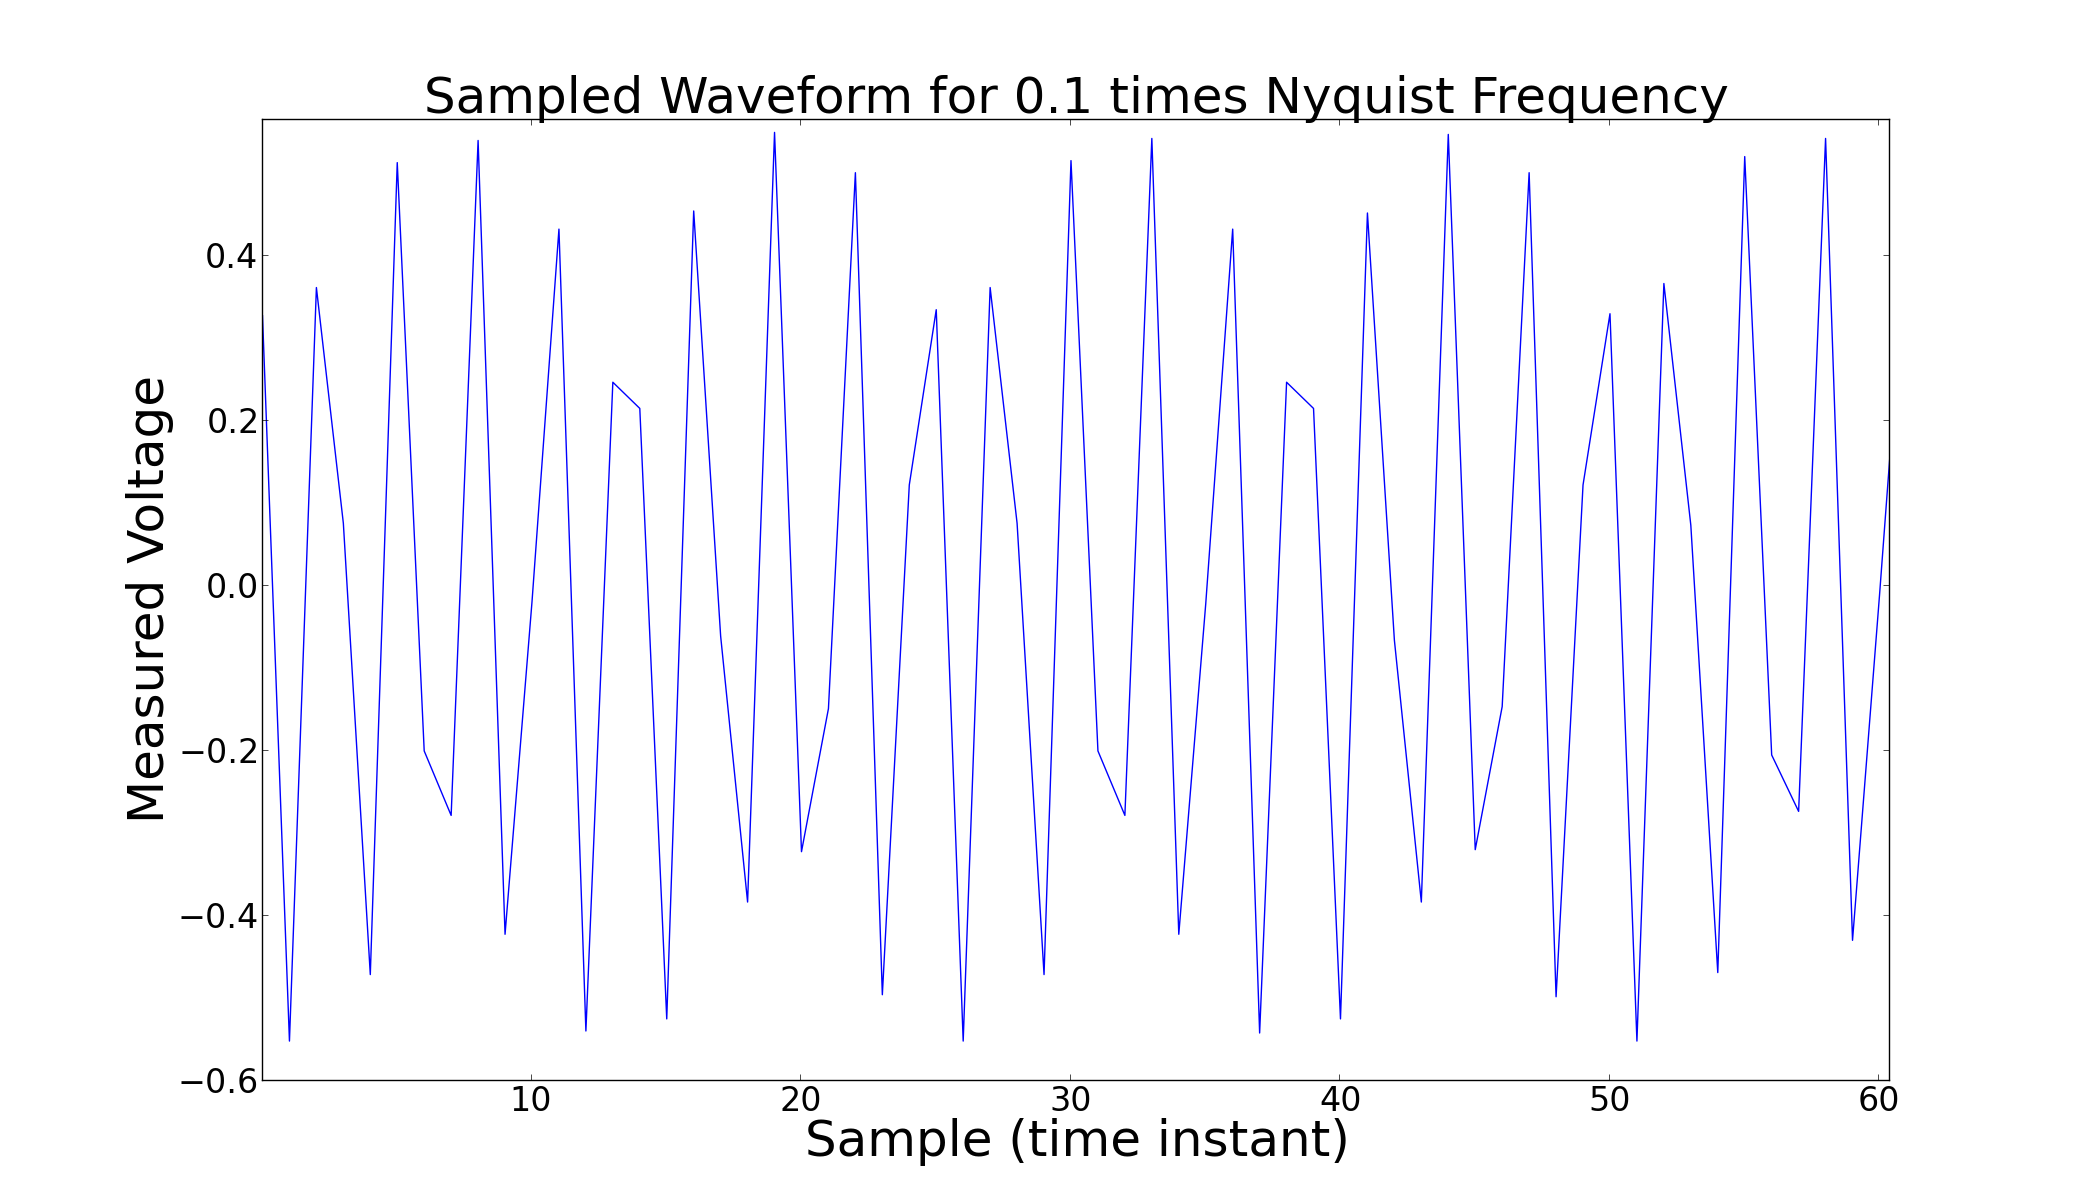
\includegraphics[scale=0.15]{pictures/pointonenyq}
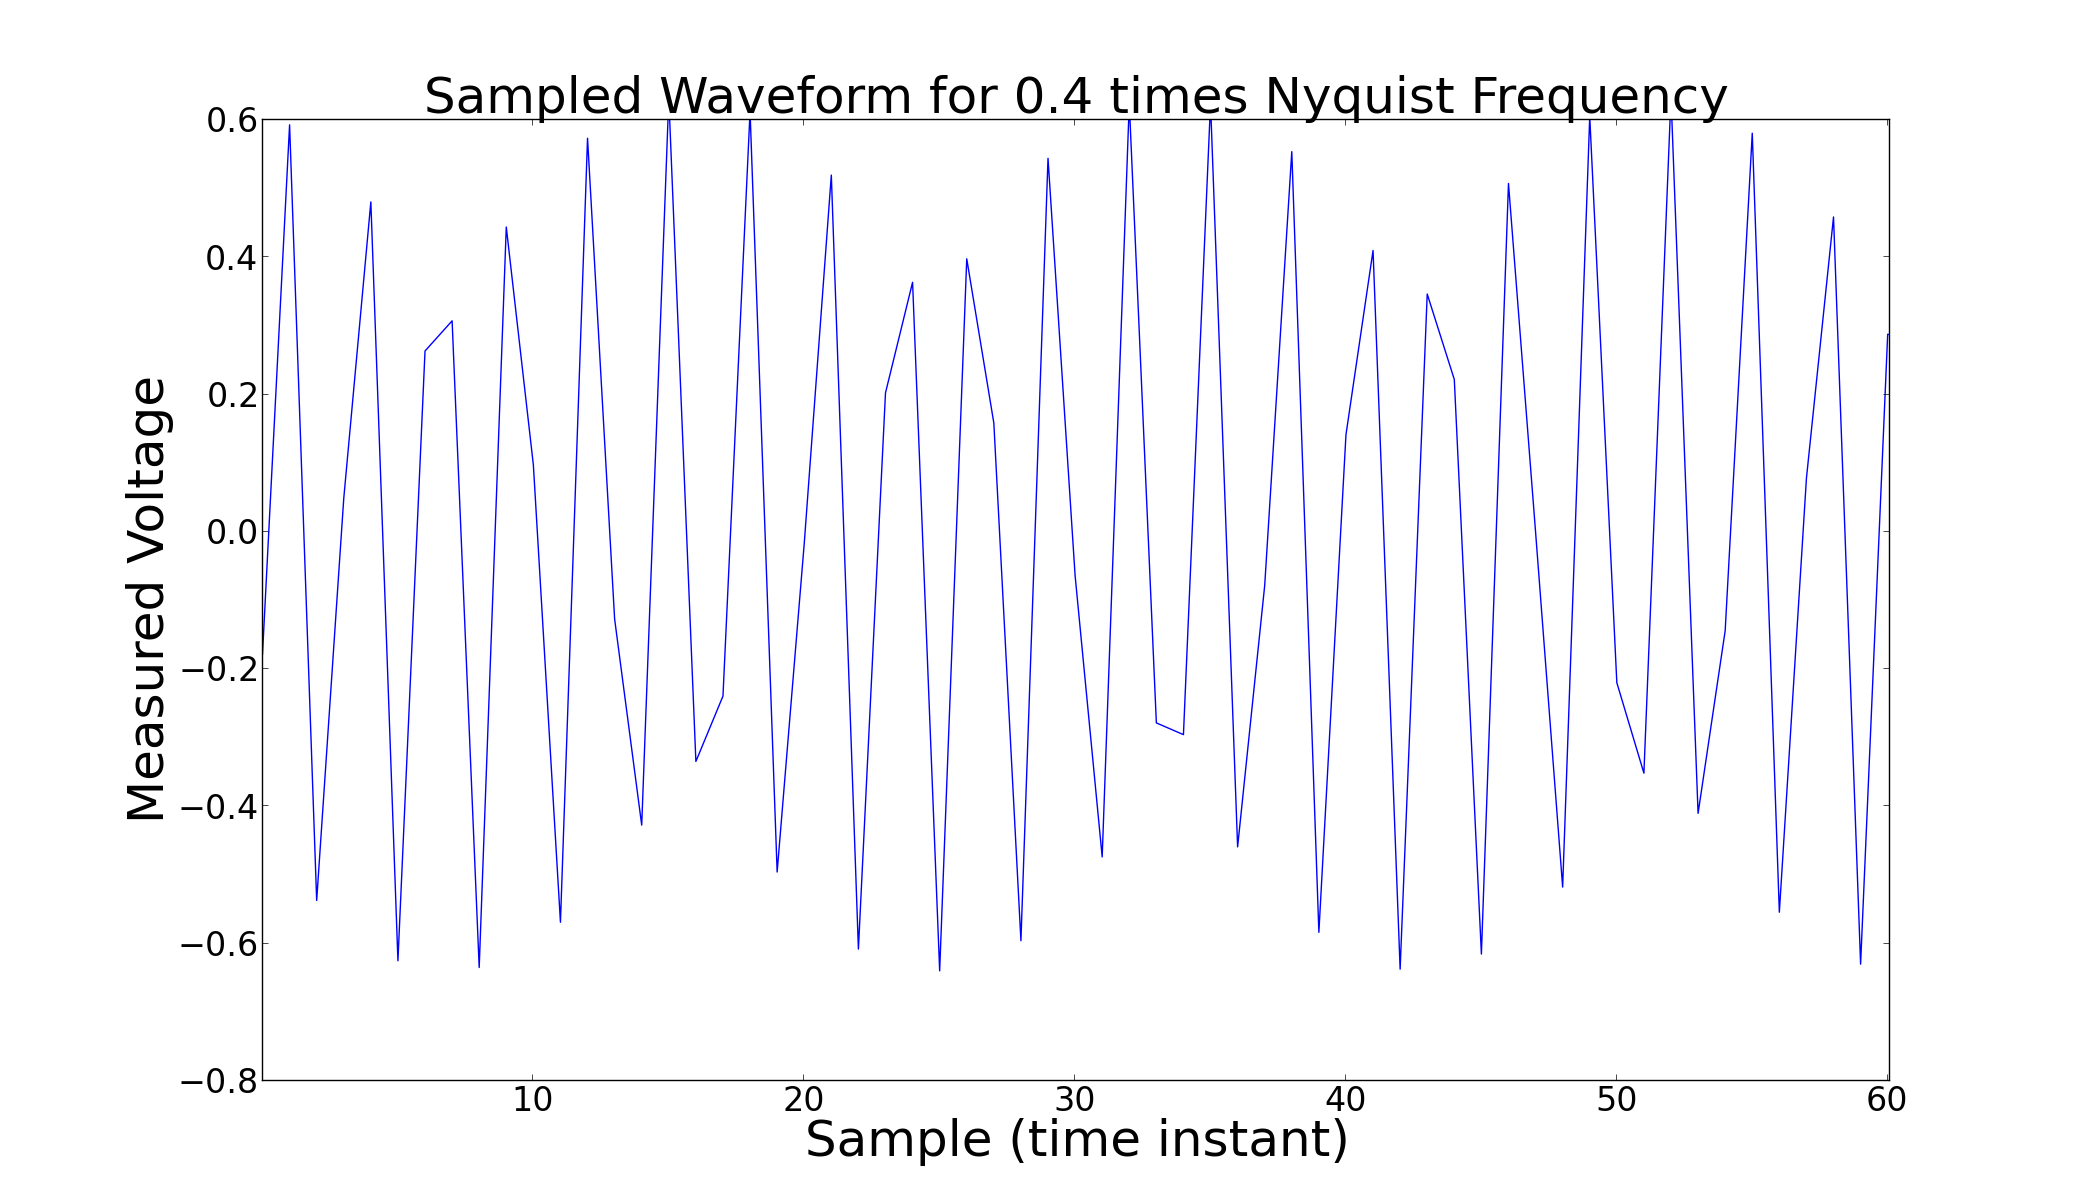
\includegraphics[scale=0.15]{pictures/pointfournyq}
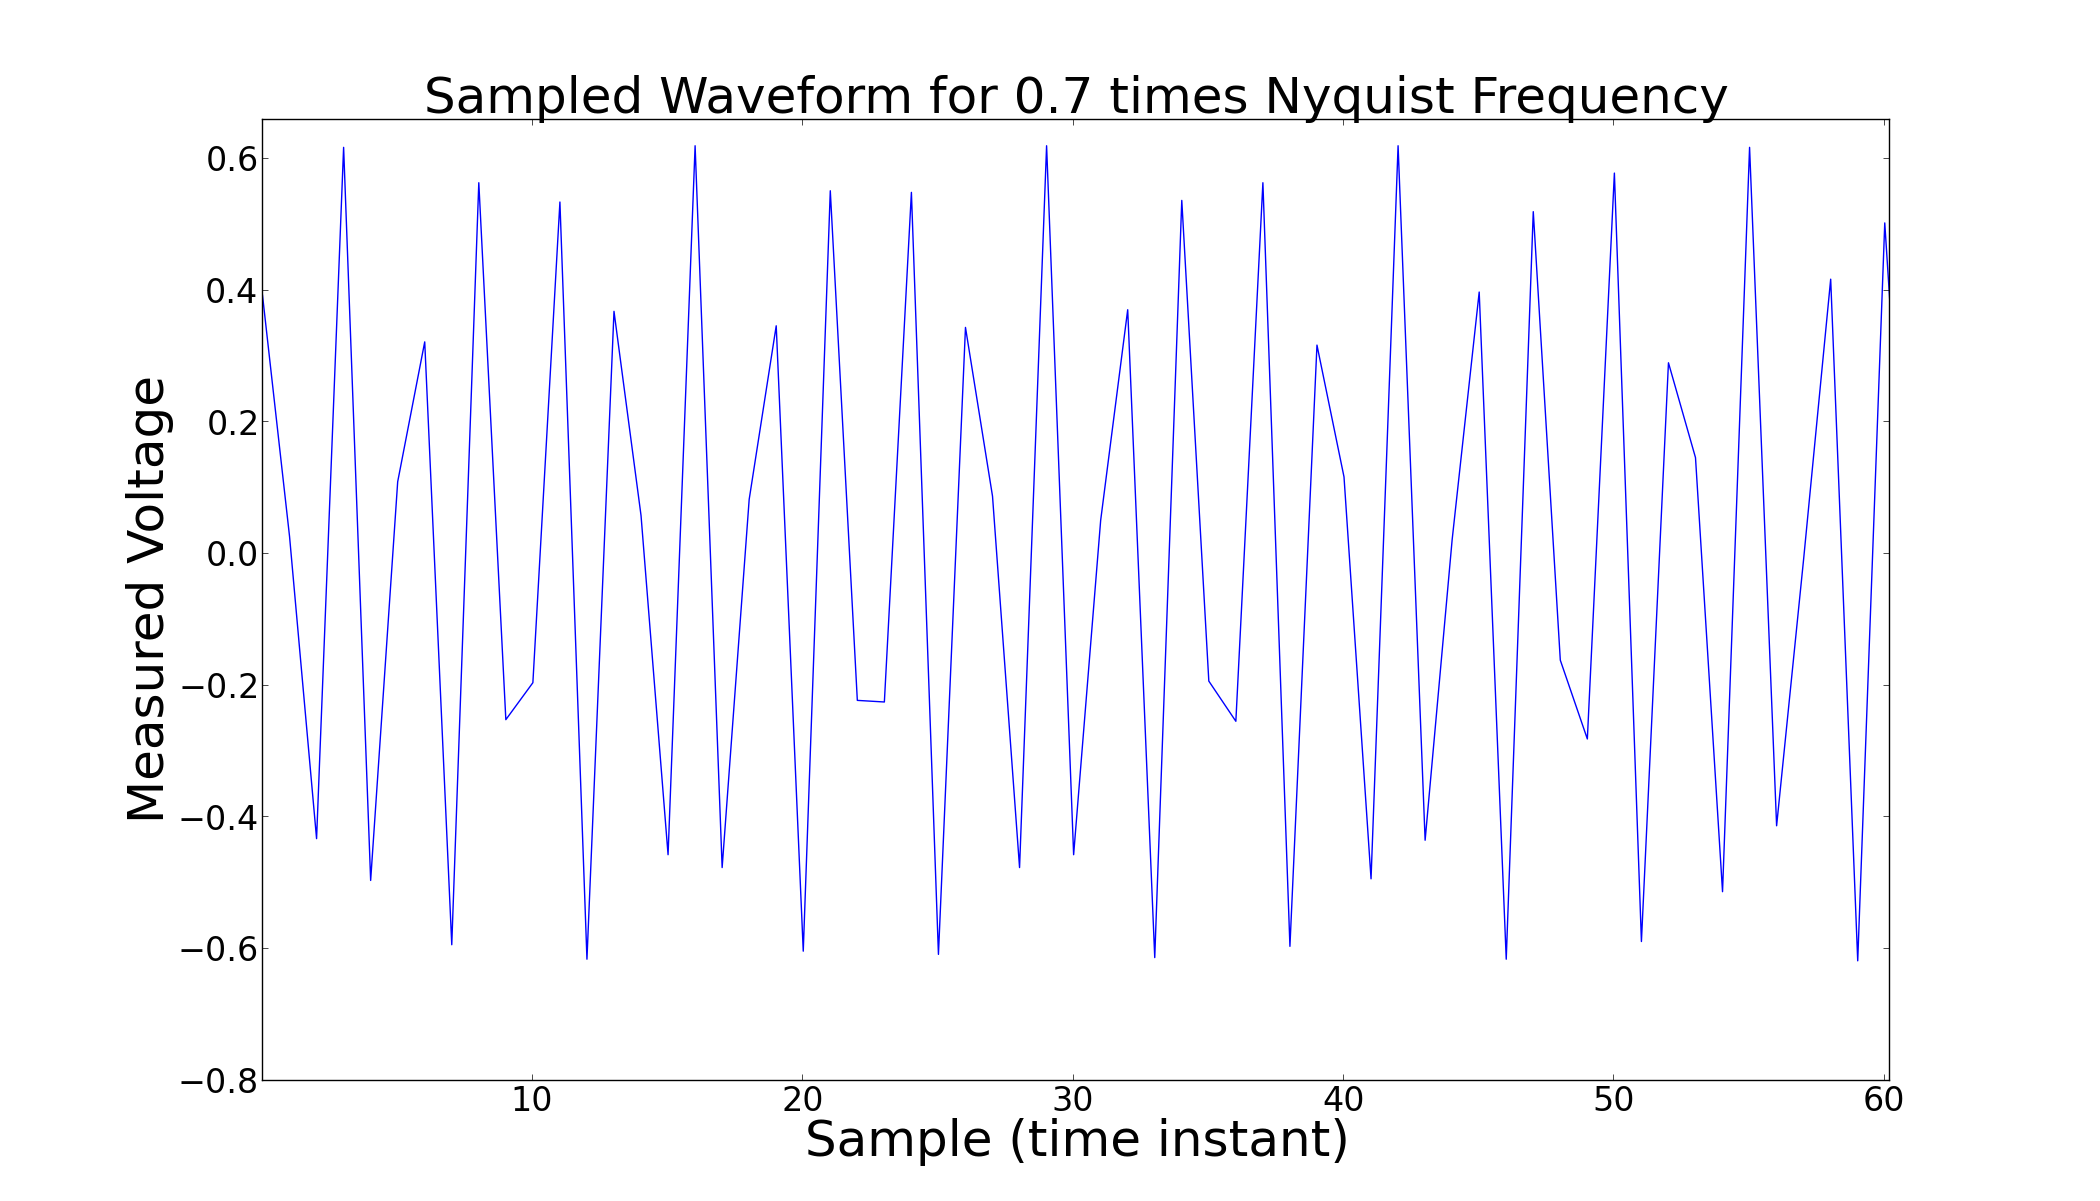
\includegraphics[scale=0.15]{pictures/pointsevennyq}
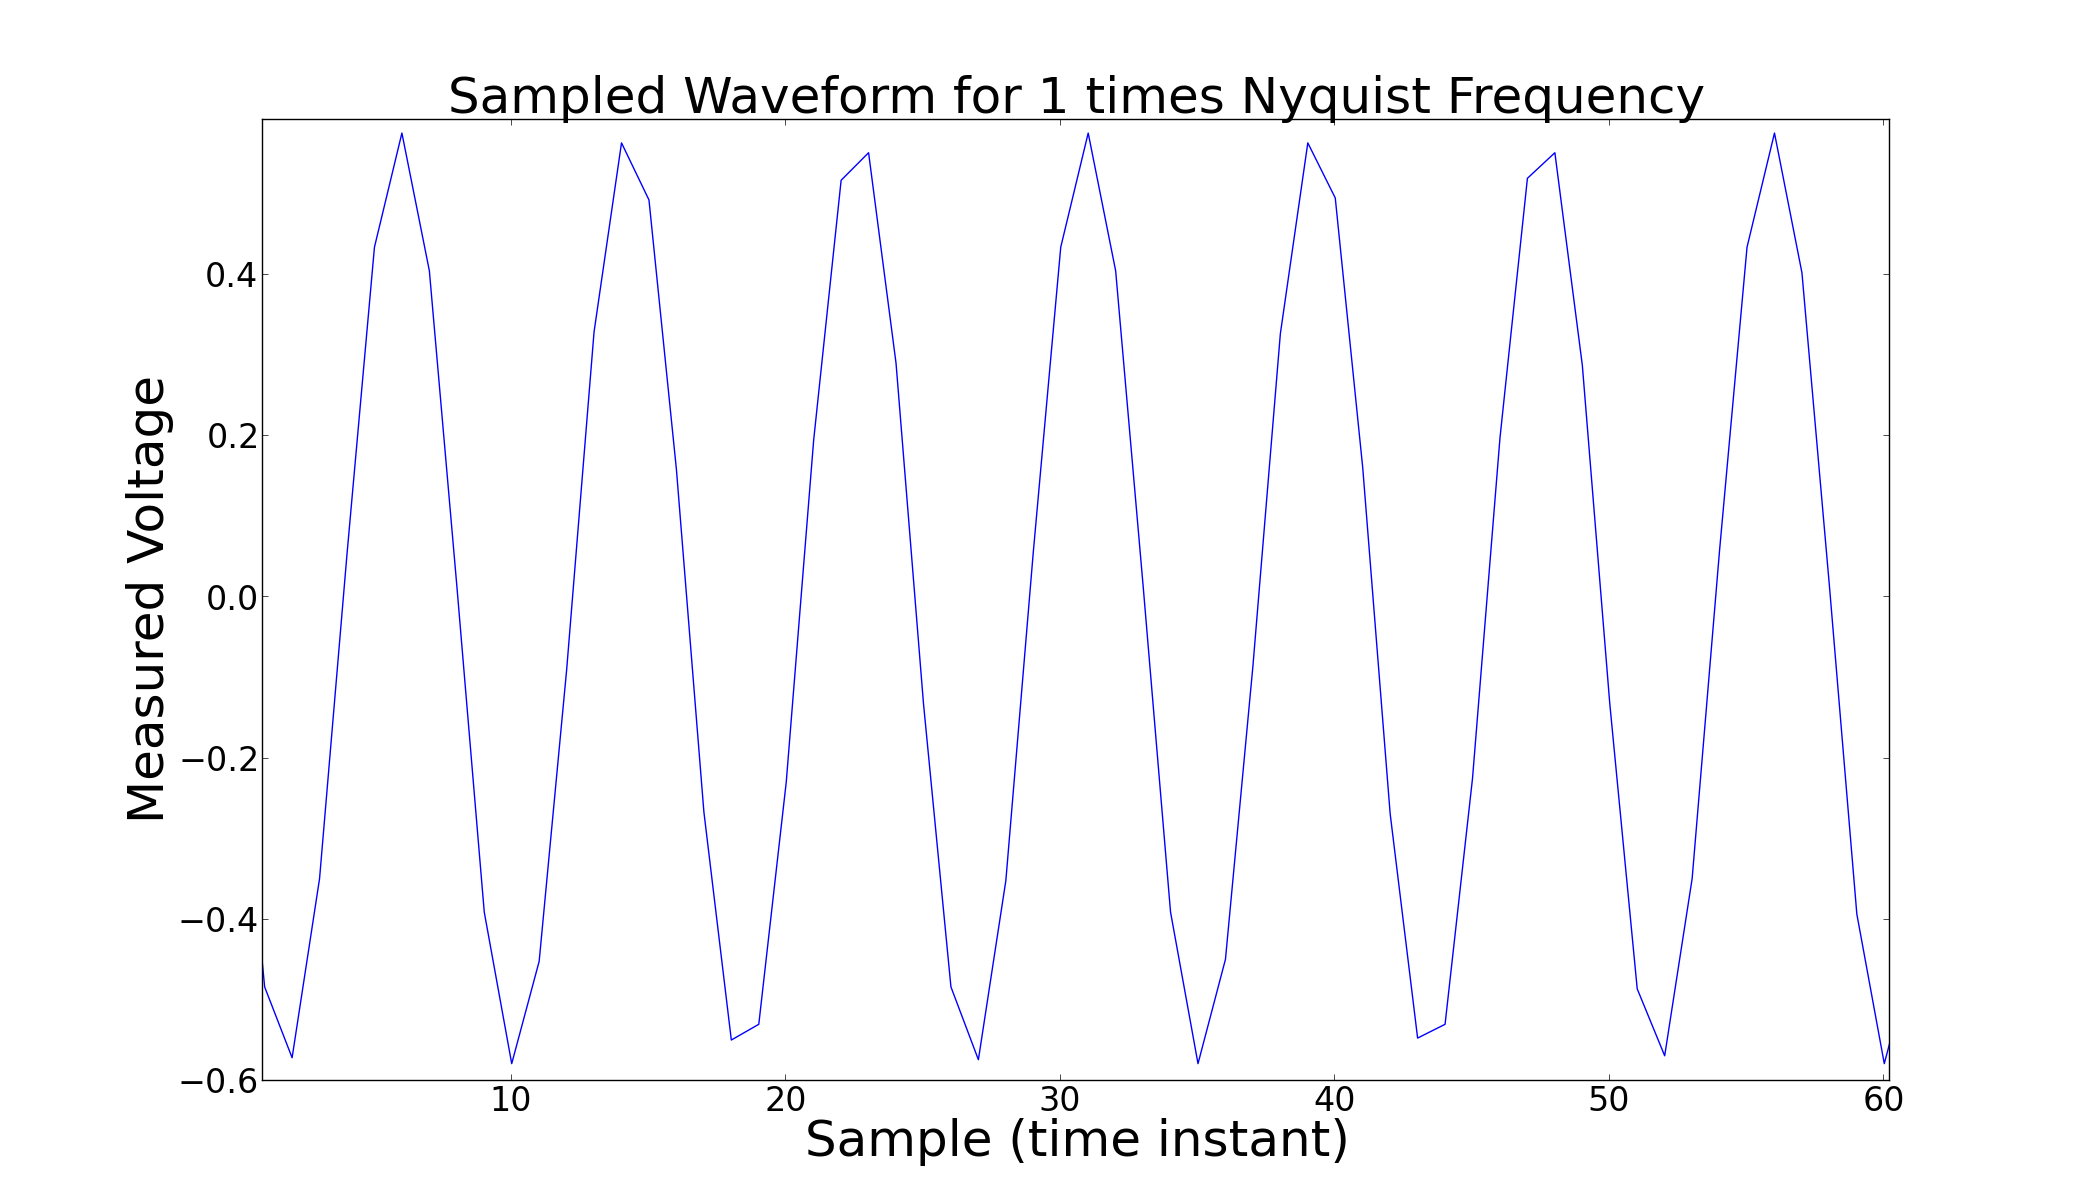
\includegraphics[scale=0.15]{pictures/onetimesnyq}
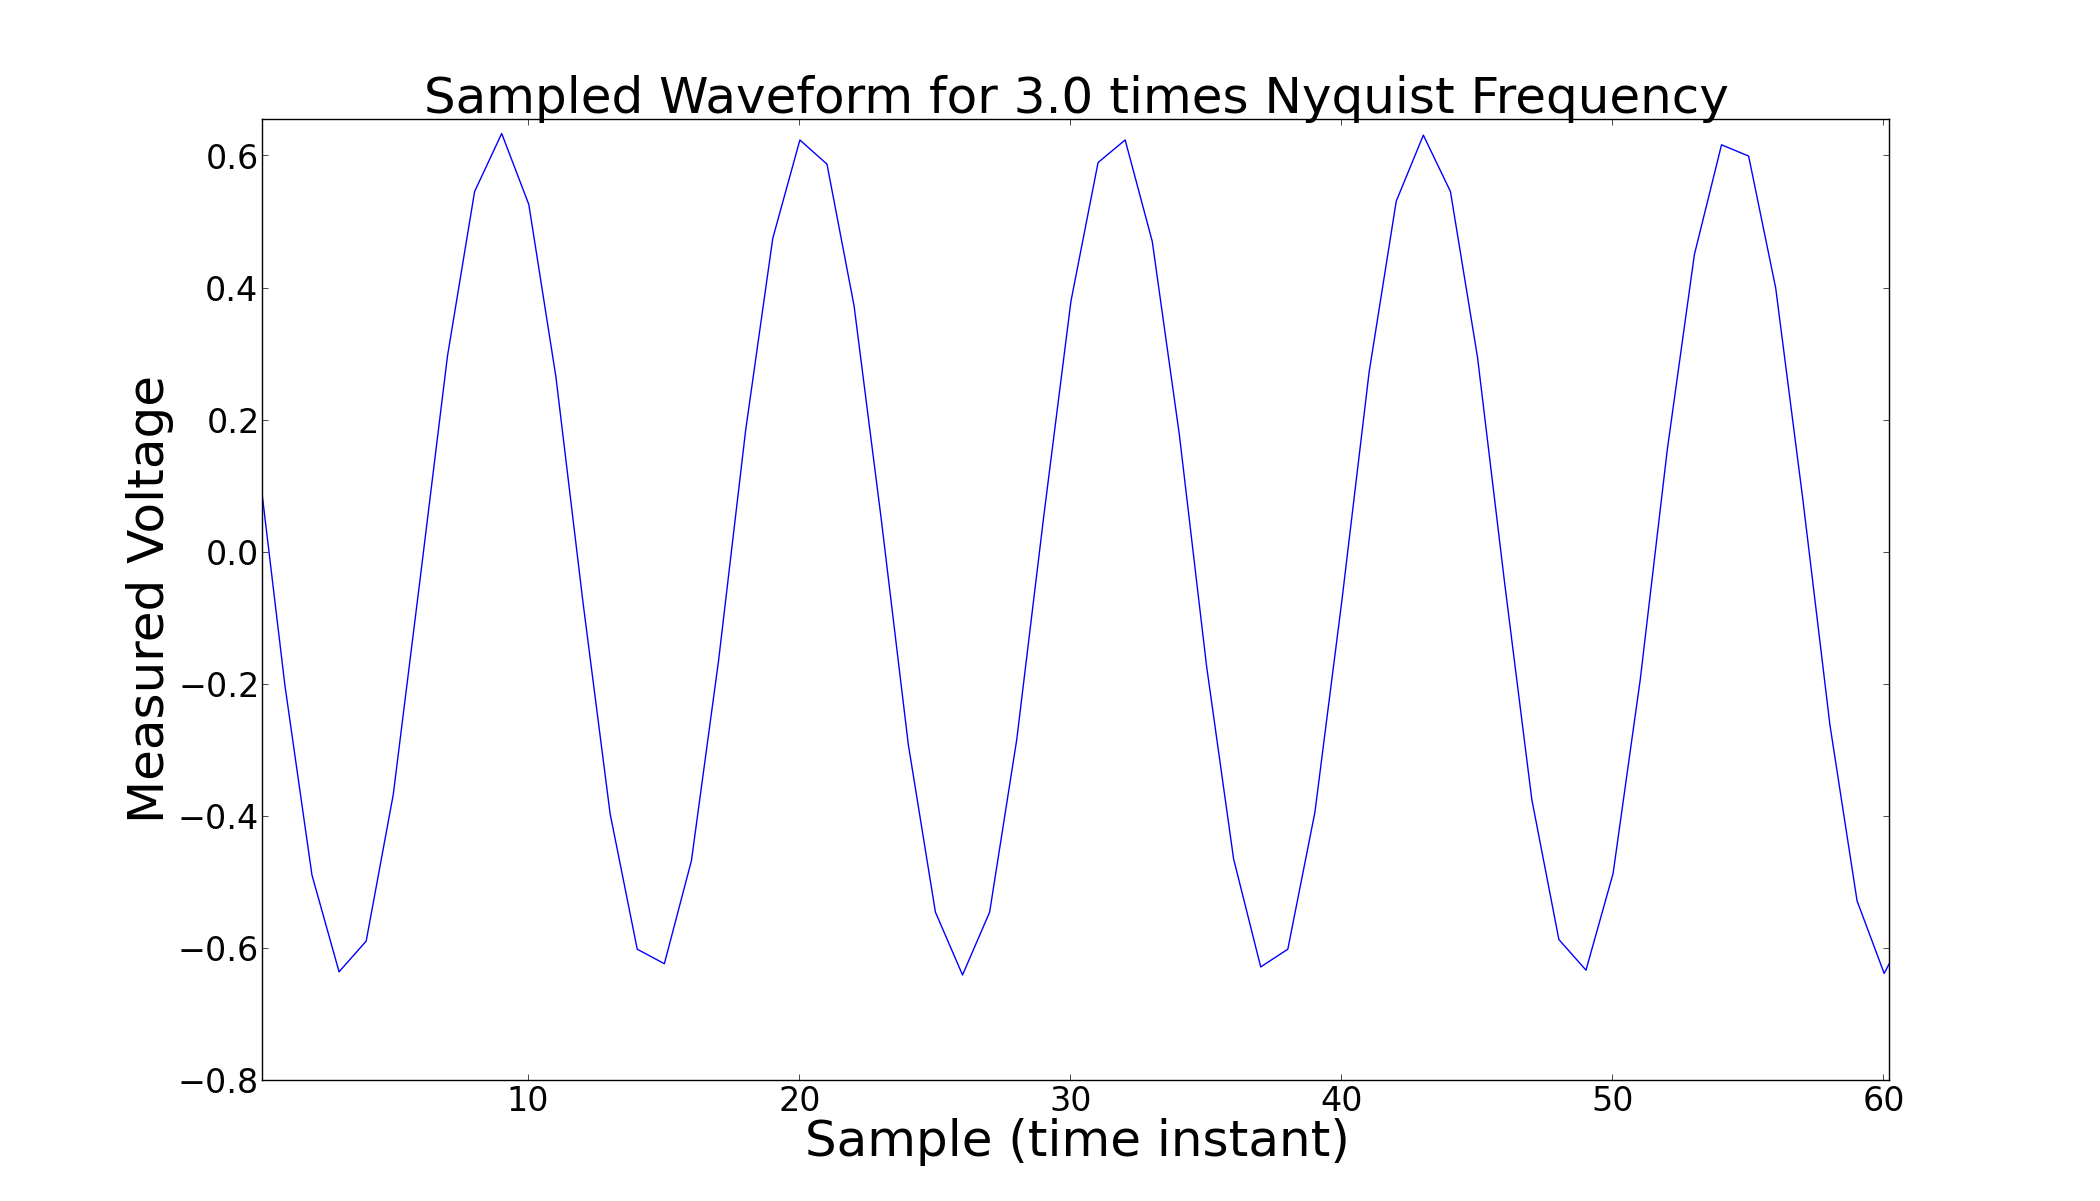
\includegraphics[scale=0.15]{pictures/triplenyq}
\caption{Sinusoidal signal sampled at 0.1, 0.4, 0.7, 1, and 3
  times Nyquist frequency. \label{nyq}}
\end{figure}

\subsection{Mixing}



%COMMENT:By placing your figures in the flow of your text, you can
%increase the likelihood that they appear in reasonable places based on
%where you reference them. Combining figures (2 & 3 were combined) that
%are related or demonstrate two aspects of one thing can also allow you
%to use space in your paper more effectively.


%COMMENT: Captions should go below figures always.

%COMMENT: In a report you don't need to write out unit names, and it
%would actually be preferred you use things like $\mu$H versus mircoHenry

\end{document}
